\subsection{Rekombination}
Im Allgemeinen wird versucht aus den Genen der Eltern, mit Hilfe von
Rekombinationsmethoden neue Chromosomen bei den Nachfolgenerationen
zu erzeugen. Nach \cite{ErbenSkript} können so, mit neuen Chromosomen
auch neue Lösungen gefunden werden. Zuerst werden hierfür nach
\cite{ErbenSkript} die im Mating-Pool befindlichen Chromosome mit
einer vorbestimmten Wahrscheinlichkeit zur Paarung ausgewählt. 
'Unter den ausgewählten Chromosomen werden zufällige Elternpaare ( parents )
gebildet', \cite{ErbenSkript}. Danach werden je nach Rekombinationsart,
die zufällig ausgewählten Gene, unter den Eltern getauscht und auf die
Nachkommen übertragen.

\subsection{Rekombinationsoperator 'recpm'}
Bei herkömmlichen Rekombinationsverfahren, wie bspw. dem 'One-Point'- oder
auch 'Two-Point'-Crossover, kann es vorkommen, dass bestimmte Gene, innerhalb
eines Chromosoms doppelt vorkommen, was in bestimmten Problemstellungen
zu illegalen Lösungen führen würde. Gerade beim TSP-Problem, bei dem
jeder Ort nur einmal besucht werden darf, können derartige Lösungen
nicht akzeptiert werden. Das folgende Beispiel verdeutlicht das entstehen
einer illegalen Lösung für das TSP-Problem, anhand des 'Two-Point'-Crossovers.
Der dabei entstehende Nachkomme 'Kind1', trägt die Gene '1', '2' und '3' doppelt
in sich.

\begin{description}
  \item[Elter1-Chrom.:] 1 2 3 | 4 5 6 | 7 8
  \item[Elter2-Chrom.:] 4 6 7 | 3 1 2 | 5 8
  \item[Kind1-Chrom.:]  1 2 3   3 1 2   7 8 
\end{description}

Um derartigen Verdopplungen und illegalen Lösungen vorzubeugen, verwendet
man das Rekombinationsverfahren 'recpm', welches für 
'Partial Matching Recombination' steht. Die von Goldberg und Lingle 
vorgeschlagene Methode ist dabei besser bekannt als 'PMX', 
\cite{Berg93}. Dabei werden ebenfalls wieder die Rekombinationsbereiche
der beiden Elternchromosome ausgetauscht und den Kindern hinzugefügt.
Die restlichen Positionen der Kindchromosome werden mit den jeweils
eigenen Genen aufgefüllt, es sei denn, dass diese bereits in den 
rekombinierten Teilen auftauchen. Ist dies der Fall, so wird die 
Abbildungsfolge, die sich aus den Rekombinationsteilen ergibt, als
Mapping benutzt, um die übrigen Gene entsprechend zu tauschen und dem
Kind an entsprechender Stelle hinzuzufügen. Das Beispiel in Abb.
\ref{fig:RECPM1} und Abb. \ref{fig:RECPM2} soll die genannten Aspekte
verdeutlichen. 

\begin{figure} 
  \centering
  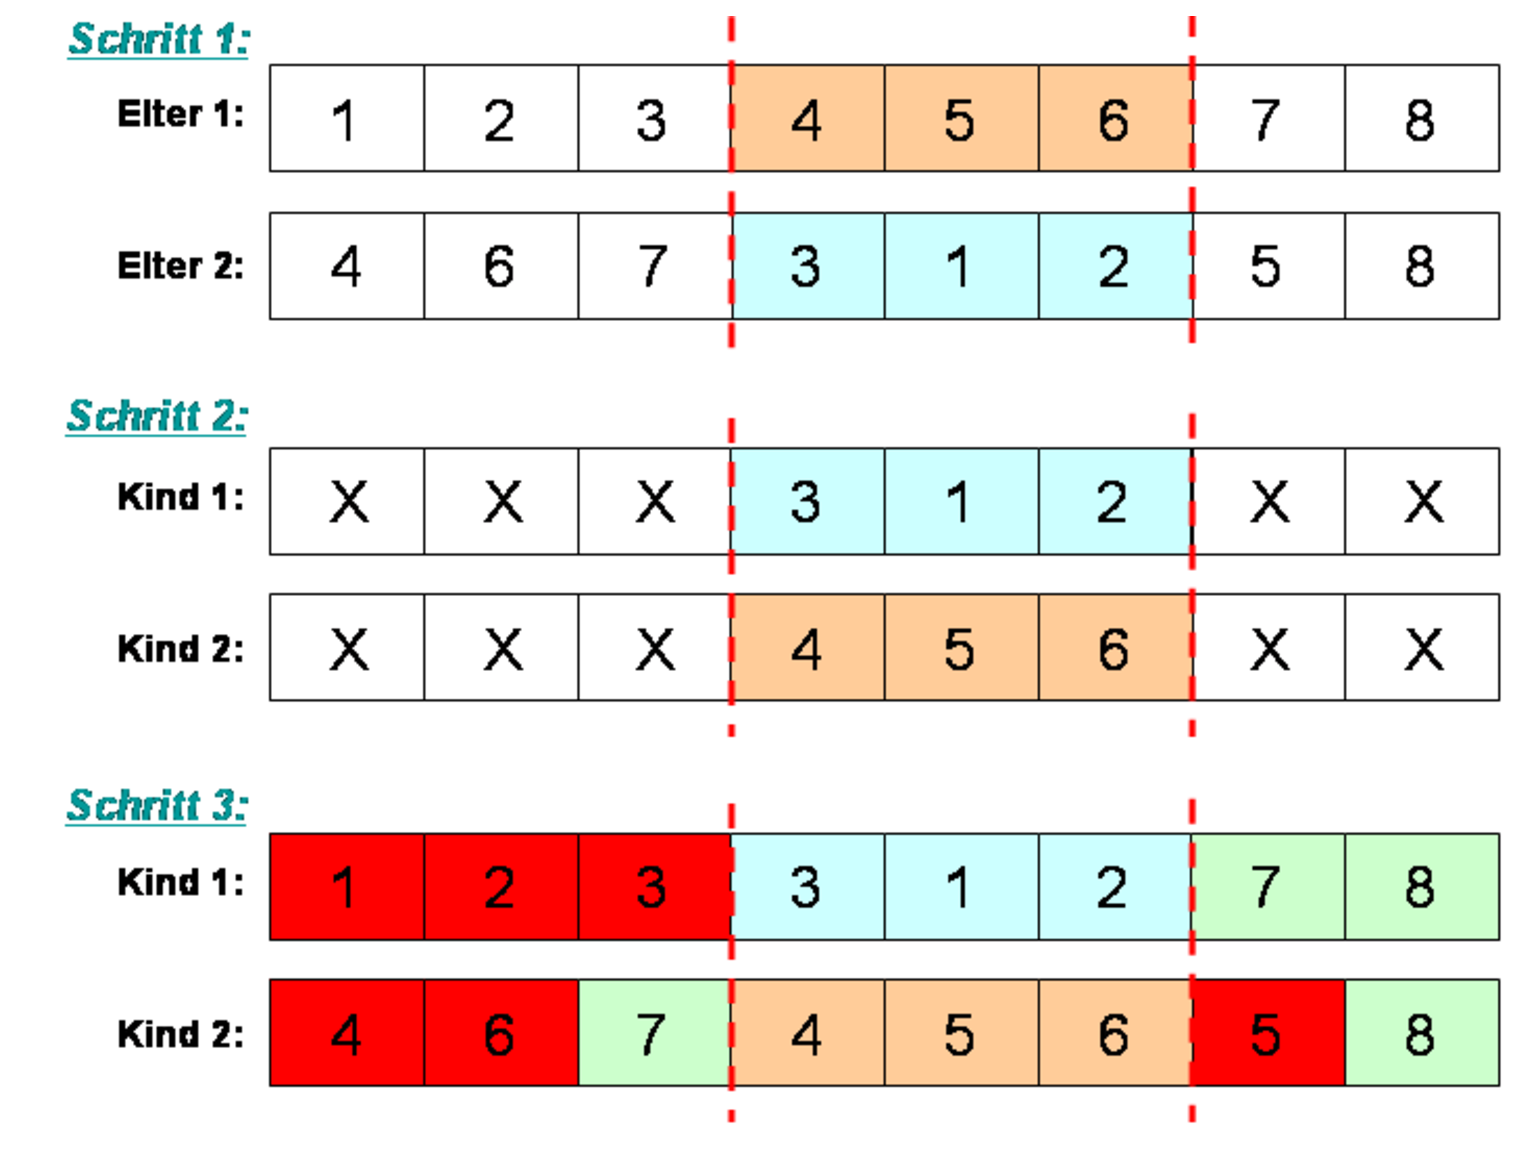
\includegraphics[width=0.8\textwidth]{../images/picRECPM1}
  \caption{Schritt 1-3 des 'Partial Recombination Crossover'}
  \label{fig:RECPM1}
\end{figure}

\begin{figure} 
  \centering
  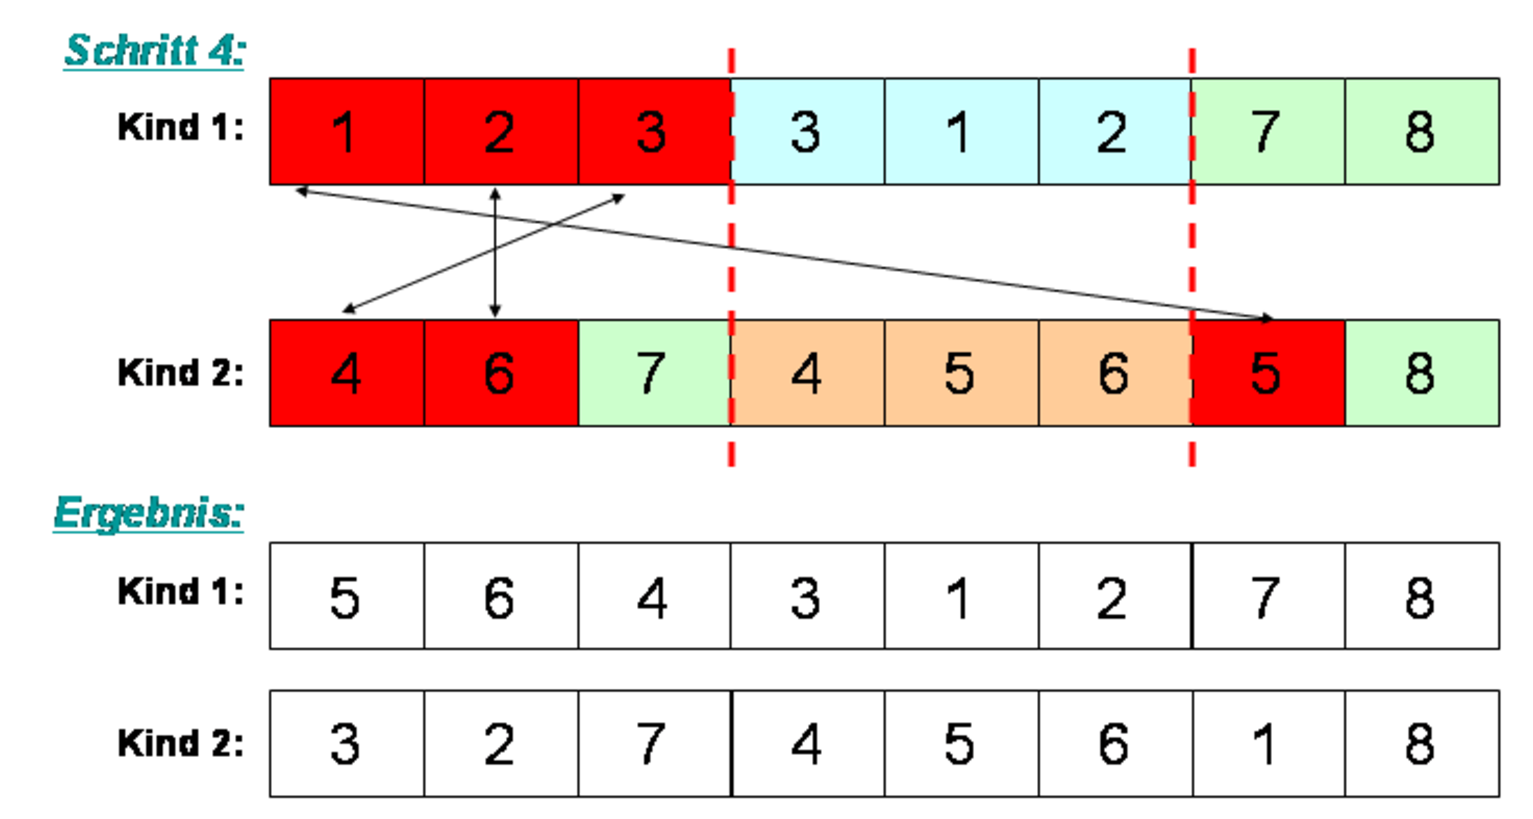
\includegraphics[width=0.8\textwidth]{../images/picRECPM2}
  \caption{Schritt 4 mit Ergebnis des 'PMX'}
  \label{fig:RECPM2}
\end{figure}

Im ersten Schritt wird der Rekombinationsbereich bestimmt. Die sich
darin befindlichen Gene werden im 2. Schritt zwischen den Eltern
ausgetauscht und den jeweiligen Kindern hinzugefügt. Die Gene
im Rekombinationsteil legen das später verwendete 'Mapping' fest
(hier 3<->4, 1<->5 und 2<->6). Im 3. Schritt
werden die Kindchromosome mit den jeweils restlichen Genen der Eltern
aufgefüllt. Die grün markierten Gene kennzeichnen dabei Werte, die
sich ohne Konflikte (Verdopplungen) hinzufügen lassen. Die rot Markierten
kennzeichnen die Gene, bei denen durch einfaches Hinzufügen ein illegaler
Zustand erreicht würde. Diese müssen über das erwähnte Mapping, gegeneinander
ausgetauscht werden. In diesem Fall wird bspw. die '1' von 'Kind1' gegen
die '5' von 'Kind2' ausgetauscht. Dieser Vorgang wiederholt sich solange, bis ein
legaler Zustand beider Chromosome erreicht ist.  

\subsection{Cycle Crossover}
Der \emph{Cycle Crossover}-Operator stellt sicher, dass die aus zwei gültigen
Elternchromosomen erzeugten Nachkommen wiederum gültige Individuen sind. Dazu
wird festgelegt, dass jedes Gen im Nachkommen von der selben Stelle eines der
Elternchromosome übernommen wird.

Der Algorithmus läuft in den folgenden Schritten ab, hier für die Erzeugung eines
Kindes $k$ aus zwei Eltern $e_1$ und $e_2$:

\begin{enumerate}
  \item Bestimmen einer zufälligen Startposition $s$.
  \item Übernehmen des Wertes an der Stelle $s$ an die selbe Stelle von $k$:
  $k[s] = e_1[s]$.
  \item Suchen der Position $i$ in $e_2$, an welcher der soeben gefundene Wert
  $e_1[s]$ steht.
  \item Übernehmen des Wertes aus $e_1$ nach $k$, welcher an der Stelle $i$
  steht: $k[i] = e_1[i]$.
\end{enumerate}

Dieser Vorgang wird solange wiederholt, bis sich ein Kreis (\emph{cycle})
gebildet hat, d.h. man zu einem bereits übernommenen Wert gelangt. Abschließend werden
die verbleibenden Stellen unverändert aus dem zweiten Elternteil übernommen.

\subsubsection{Implementierung in Matlab}
Listing \ref{lst:reccycle} zeigt unsere Implementierung des Cycle
Crossover-Operators in Matlab. Dabei haben wir die Struktur der Funktion
übernommen aus einer der GEATbx beiliegenden Operator-Funktionen, nämlich der
\texttt{recmp.m}.

\lstinputlisting[caption={Implementierung Cycle Crossover in Matlab},
label={lst:reccycle}]{../reccycle.m}

\subsection{Testläufe mit variierenden Rekombinations-Methoden}
Um die verschiedenen Rekombinationsoperatoren zu testen, wurden jeweils 20
Testläufe mit den folgenden Einstellungen vorgenommen:

\begin{description}
  \item[Anzahl Subpopulationen:] 12
  \item[Anzahl Individuen:] 60
  \item[Selektionsoperator:] Tournament-Selektion, \texttt{seltour}
  \item[Mutationsoperator:] Kombination aus \texttt{mutswap}, \texttt{mutmove} 
	und \texttt{mutinvert}
  \item[Rekombinationsoperator:] Variation zwischen \texttt{recgp},
  \texttt{recpm} und dem eigenimplementierten \texttt{reccycle}
\end{description}

Tabelle \ref{tbl:aufgabeE-ergebnisse} zeigt die Ergebnisse der Testläufe. 

\begin{table}
	\sffamily
	\centering
	\footnotesize
	\begin{tabularx}{\textwidth}{TlllllX}
		\toprule
		\multicolumn{1}{@{}N}{Rekombination} &
		\multicolumn{1}{V{5em}@{}}{Mittelwert $\bar{x}$} &
		\multicolumn{1}{V{6.5em}@{}}{Standardabw. $\sigma_x$} &
		\multicolumn{1}{V{9em}@{}}{Minimalwert in Lauf $r$, Generation $g$} &
		\multicolumn{1}{V{9em}@{}}{Maximalwert in Lauf $r$, Generation $g$} & 
		\multicolumn{1}{V{5em}@{}}{Mittelwert CPU-Zeit [s]} \\
		\midrule\addlinespace
		recgp & 2201,50 & 106,00 & 2035, $r = 11$, $g = 100$ & 2353, $r = 1$, $g
		= 100$ & 131,31\\
		\midrule
		recpm & \textbf{2195,45} & 97,81 & \textbf{2034}, $r = 1$, $g = 82$ & 2358, $r = 19$, $g = 98$ & 31,95\\
		\midrule
		reccycle & 2302,30 & \textbf{89,05} & 2147, $r = 6$, $g = 96$ & 2449, $r = 3$, $g = 98$ & 19,65\\

		\addlinespace\bottomrule
		\end{tabularx}
	\caption{Zusammengefasste Ergebnisse der Testreihe}
	\label{tbl:aufgabeE-ergebnisse}
\end{table}
 
\subsubsection{Interpretation der Ergebnisse}
Wie man an den Ergebnissen der Testreihe ablesen kann, scheint es zwischen den
einzelnen Rekombinationsoperatoren keine signifikanten Unterschiede zu geben. Das
beste Mittelwertergebnis dieser Testreihe mit ca. 2195 km wurde unter Verwendung
des \texttt{recpm}-Verfahrens erreicht. Der von uns implementierte
\texttt{reccycle}-Operator schnitt bei den Mittelwerten schlechter ab, jedoch
erzielte er die geringsten Standardabweichung in der Testreihe. Was man
allerdings festhalten muss, ist die Tatsache, dass \texttt{recgp} einen erheblich
höheren CPU-Aufwand erfordert als der \texttt{reccycle}-Operator. Hier sind
benötigte Ergebnis-Güte und Rechenzeit gegeneinander abzuwägen. Abbildung
\ref{fig:aufgabeE-plot} zeigt nochmals den kompletten Verlauf der Testergebnisse
in graphischer Form.

\begin{figure}
  \centering
  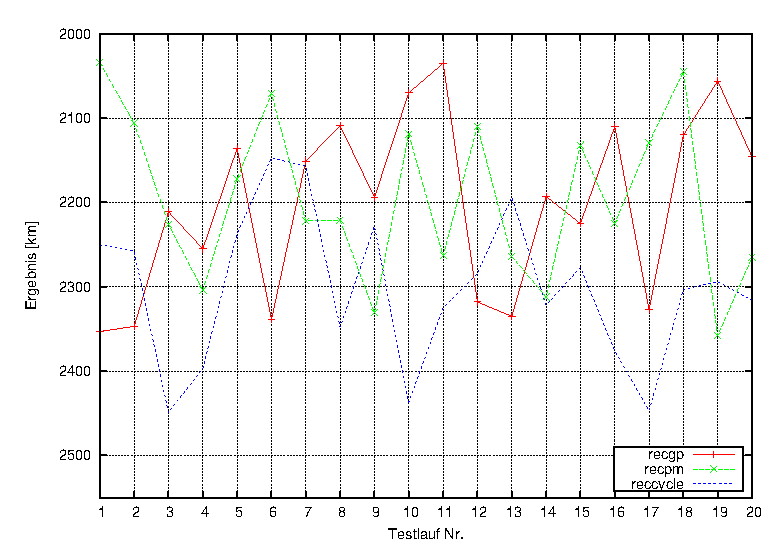
\includegraphics[width=1.0\textwidth]{../images/aufgabeE-plot}
  \caption{Grafische Darstellung der Testreihe mit verschiedenen Rekombinationsoperatoren}
  \label{fig:aufgabeE-plot}
\end{figure}